\documentclass[a4paper, 10pt, conference]{ieeeconf}

\IEEEoverridecommandlockouts

\overrideIEEEmargins

\usepackage{amssymb,url,amsmath}
\usepackage{algorithm}
\usepackage{graphicx}
\usepackage{epstopdf}
\usepackage{textcomp}
\usepackage{color}
\usepackage{ifpdf}
\usepackage{url}
\usepackage{enumerate}
\usepackage{array}
\usepackage{flushend}
\usepackage{multirow,booktabs}
\usepackage{hyperref}
\usepackage{subfig}
\usepackage{mdwlist}
\usepackage[utf8]{inputenc}
\usepackage{tcolorbox}
\newcommand{\alg}{Algorithm~}
\newtcolorbox[auto counter]{algorithmbox}[2][]{colback=red!5!white,colframe=red!75!black,fonttitle=\bfseries, title=\alg\thetcbcounter: #2,#1}

\newcommand{\eq}{Eq.~}
\newcommand{\fig}{Fig.~}
\newcommand{\tab}{Tab.~}
\newcommand{\sect}{Sec.~}

\newcommand{\re}{R}
\newcommand{\rf}{R}
\newcommand{\rl}{L}
\newcommand{\om}{O}
\newcommand{\cm}{M}
\newcommand{\fm}{F}
\newcommand{\hc}{C}
\newcommand{\qd}{Q}
\newcommand{\gpm}{T}
\newcommand{\coll}{W}
\newcommand{\pdf}{\mathbf{pdf}}

\newcommand{\argmax}[1]{\underset{#1}{\operatorname{argmax}}\medspace}

\graphicspath{{images/}}

\title{\LARGE \bf
Learning and Inference of Dexterous Grasps for Novel Objects with Underactuated Hands
}

\author{Marek Kopicki$^{1}$ and Carlos J. Rosales$^{2}$ and Hamal Marino$^{2}$ and Marco Gabiccini$^{2}$ and Jeremy L. Wyatt$^{1}$% <-this % stops a space
\thanks{*This work was supported by EC-FP7-ICT-600918, PacMan.}% <-this % stops a space
\thanks{$^{1}$Marek Kopicki and Jeremy L. Wyatt are with the Intelligent Robotics Laboratory, School of Computer Science,
        University of Birmingham, Birmingham, B15 2TT, UK.}
        %{\tt\small \{msk,jlw\}@cs.bham.ac.uk}}%
\thanks{$^{2}$Carlos J. Rosales, Hamal Marino and Marco Gabiccini are with Centro Piaggio, Universita di Pisa, Pisa, Italy.}
               %{\tt\small carlos.rosales@for.unipi.it, hamal.marino@centropiaggio.unipi.it, m.gabiccini@ing.unipi.it}}%
\thanks{Correspond to: {\tt\small M.S.Kopicki at cs.bham.ac.uk}}%
}
\begin{document}


\maketitle
\thispagestyle{empty}
\pagestyle{empty}


%%%%%%%%%%%%%%%%%%%%%%%%%%%%%%%%%%%%%%%%%%%%%%%%%%%%%%%%%%%%%%%%%%%%%%%%%%%%%%%%
\begin{abstract}
Recently, advances have been made in learning of grasps for fully actuated hands. A typical approach is to learn the target locations of finger links on the object surface. When a new object must be grasped, new finger locations are generated, and a collision free reach-to-grasp trajectory is planned. Such a division of labour fails to exploit the advantages of underactuated hands, which improve grasp reliability via contacts with the object during grasping. In this paper we present a method for learning grasps for underactuated hands. Our approach works by learning not only the desired final grasp, but also good grasping trajectories. We learn these trajectories from example grasps generated with a rigid body simulation of hand and object. This enables us to learn how to approach the object and close the underactuated hand so as to induce a favourable sequence of contacts. Our method does not rely on explicit representation of the contact sequence. The core learning method uses a product of experts approach. This allows grasp transfer to novel objects and works despite partial shape reconstruction.
\end{abstract}


%%%%%%%%%%%%%%%%%%%%%%%%%%%%%%%%%%%%%%%%%%%%%%%%%%%%%%%%%%%%%%%%%%%%%%%%%%%%%%%%
\section{INTRODUCTION}
\label{sec:introduction}
Transferring dexterous grasps to novel objects is a challenging problem. One approach is to machine learn solutions with techniques able to perform powerful generalisation. Another is to use an underactuated hand to cope with shape variation. In this paper we combine the benefits of both approaches by learning grasps for underactuated hands. Underactuated hands exploit the contacts that occur during grasping to achieve a wide variety of final grasp configurations. The final grasp configuration depends not only on the final hand pose, but also on the object shape, and on the reach to grasp trajectory. An interesting challenge is to use machine learning to exploit these interactions. The key technical challenge in applying machine learning to grasping with underactuated hands is to learn the right motor actions so as to learn contact interactions that will lead to a reliable final grasp.

\begin{figure}
  \centering
  \begin{tabular}{ccc}
  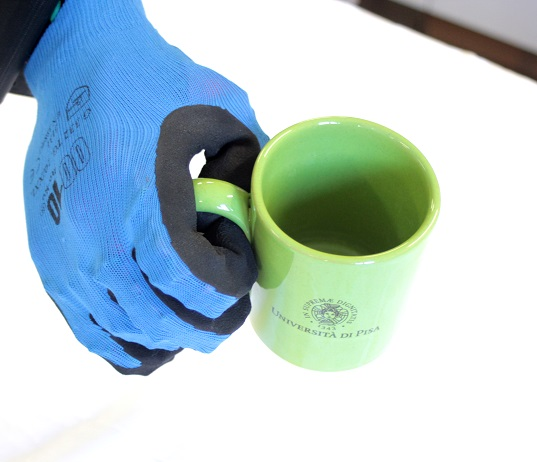
\includegraphics[width=0.45\linewidth]{mug_1_small.jpg} &
  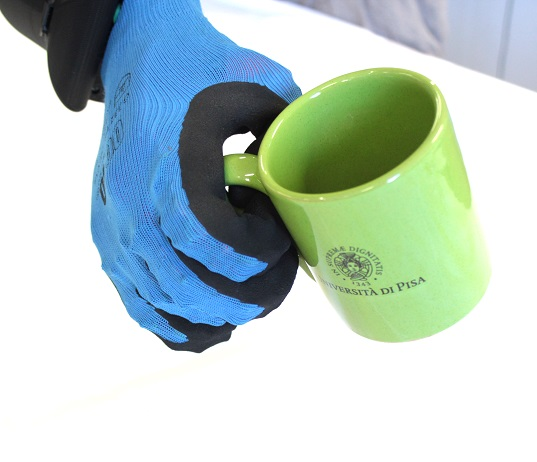
\includegraphics[width=0.45\linewidth]{mug_2_small.jpg} \\
  \end{tabular}
 \caption{{We want transferrable grasps that are robust to different initial hand-object poses, and thus different interactions during reach to grasp, thus reaching similar final grasp states. We achieve this by learning a set of trajectories that, associated with a model of the final grasp state, form an attractor basin around that state.}}
  \label{fig:two_grasps}
\end{figure}

One approach would be to explicitly learn the typical contact interactions that occur during a grasp, and to generate new grasps that reproduce these. The contact interactions are, however, complex and variable, even given small variations in object shape and friction. This makes transfer learning for underactuated hands challenging. There are two main novel technical contributions. First, we extend our learning method, so as to learn a grasp type from multiple trajectories. Second we implicitly encode the sequence of contact interactions by remembering the motor commands for finger closing as well as the wrist trajectory. We also demonstrate, for the first time, learning from examples generated in a rigid body physics simulation. Finally, at the grasp selection stage we now optimise across a space defined by several examples so as to maximise the chance of reaching a stable grasp. The method copes with partial and noisy shape information for the test objects. 

% SUBSECTION BETTER?

\subsection{Related Work}
Previous work in learning generalisable grasps falls broadly into two classes. One class of approaches utilises the shape of common object parts or their appearance to generalise grasps across object categories \cite{saxena2008b,detry2013a,herzog2014a, kroemer2012a}. This works well for low DoF hands. Another class of approaches captures the global properties of the hand shape either at the point of grasping, or during the approach \cite{ben2012generalization}. This global hand shape can additionally be associated with global object shape, allowing generalisation by warping grasps to match warps of global object shape \cite{hillenbrand2012transferring}. This second class works well for high DoF hands, but generalisation is more limited. We have previously achieved the advantages of both classes, generalising grasps across object categories with high DoF hands. In this paper we go beyond this, learning and generalising grasps for under-actuated hands.

Several hands with such behavior have been proposed in the literature with different implementations~\cite{Catalano2014Adaptive, Dollar2010Highly}, with a common goal: simplicity plus robustness. Their initial tests under human operation are promising, but autonomous grasping with underactuated hands faces challenges due to the almost non-observability of the finger deformation when the hand is constrained by the environment and/or a target object. Most of the existing planning algorithms for this type of hands boil down to generating good wrist poses and let the adaptive mechanism handle all variation and uncertainty while closing, such as~\cite{Eppner2015Planning}, where a sequence of wrist and object poses and the corresponding interaction wrenches are generated, which are expected to exploit environmental constraints. Another approach is that by~\cite{Bonilla2015Grasp}, where static wrist poses are sampled using different strategies around the object from where the fingers are closed using a rigid-body simulator, to finally select the areas of major success rate to generate new wrist poses.

While these approaches exploit, to some extent, the adaptive properties of the underactuated mechanism, they can be improved on. In this paper we show how we can, for the first time, learn grasps for underactuated hands that are then transferred to novel objects. This requires learning representations of the final grasp state that are amenable to transfer to new objects, grouping example grasps by the end grasp state, and learning and optimisation of reach-to-grasp trajectories.


%!TEX root = dexterous-grasping-sage-style.tex

\section{Representations}
\label{sec:representations}
We now sketch the representations underpinning our approach. We define several models: an object model (partial and acquired from sensing); a model of the contact between a finger link and the object; a model of the whole hand configuration; and a model of the reach to grasp trajectory. First we describe the kernel density representation for all these models. Then we describe the surface features we use to encode some of these models. We assume that the robot's hand comprises $N_L$ rigid \emph{links}: a palm, and several phalanges or links. We denote the set of links $L =\{L_i\}$.

\subsection{Kernel Density Estimation}
\label{sec:kde}
$SO(3)$ denotes the group of rotations in three dimensions. A feature belongs to the space $SE(3) \times \mathbb R^2$, where $SE(3) = \mathbb R^3 \times SO(3)$ is the group of 3D \emph{poses}, and surface descriptors are composed of two real numbers. We extensively use probability density functions (PDFs) defined on $SE(3) \times \mathbb R^2$.  We represent these PDFs non-parametrically with a set of $K$ features (or particles) $x_j$
\begin{equation}
S = \left\lbrace x_j : x_j \in \mathbb R^3 \times SO(3) \times \mathbb R^2 \right\rbrace_{j \in [1,K]}.
\end{equation}
The probability density in a region is determined by the local density of the particles in that region. The underlying PDF is created through \emph{kernel density estimation} \cite{silverman1986a}, by assigning a kernel function $\mathcal{K}$ to each particle supporting the density, as
\begin{equation}\label{eq:d}
\pdf(x) \simeq \sum_{j=1}^K w_j \mathcal{K}(x| x_{j}, \sigma),
\end{equation}
where  $\sigma \in \mathbb R^3$ is the kernel bandwidth and $w_j \in \mathbb R^{+}$ is a weight associated to $x_j$ such that $\sum_j w_j = 1$. We use a kernel that factorises into three functions defined by the separation of $x$ into $p \in \mathbb R^3$ for position, a quaternion $q \in SO(3)$ for orientation, and $r \in \mathbb R^2$ for the surface descriptor. Furthermore, let us denote by $\mu$ another feature, and its separation into position, orientation and a surface descriptor. Finally, we denote by $\sigma$ a triplet of real numbers:
\begin{subequations}
\begin{align}
x &= (p, q, r),\\
\mu &= (\mu_p, \mu_q, \mu_r),\\
\sigma &= (\sigma_p, \sigma_q, \sigma_r).
\end{align}
\label{eq:feature}
\end{subequations}
We define our kernel as
\begin{equation}\label{eq:kernel_in_se3}
\mathcal{K}(x| \mu, \sigma) = \mathcal{N}_3(p| \mu_p, \sigma_p) \Theta(q| \mu_q, \sigma_q) \mathcal{N}_2(r| \mu_r, \sigma_r)
\end{equation}
where $\mu$ is the kernel mean point, $\sigma$ is the kernel bandwidth, $\mathcal{N}_n$ is an $n$-variate isotropic Gaussian kernel, and ${\Theta}$ corresponds to a pair of antipodal von Mises-Fisher distributions which form a Gaussian-like distribution on $SO(3)$ \cite{fisher1953a,sudderth2006a}. The value of ${\Theta}$ is given by
\begin{equation}
\Theta(q|\mu_q, \sigma_q) = C_4(\sigma_q) \frac {e^{\sigma_q \; \mu_q^T q} + e^{-\sigma_q \; \mu_q^T q}}2
\end{equation}
where $C_4(\sigma_q)$ is a normalising constant, and $\mu_q^T q$ denotes the quaternion dot product.

Using this representation, conditional and marginal probabilities can easily be computed from \eq\eqref{eq:d}. The marginal density $\pdf(r)$ is computed as
\begin{align}\label{eq:marginal}
\pdf(r) & \\
      = & \iint \sum_{j=1}^K w_j \mathcal{N}_3(p| p_i, \sigma_p) \Theta(q| q_i, \sigma_q) \mathcal{N}_2(r| r_i, \sigma_r) \textnormal{d}p\textnormal{d}q \\
      = &  \sum_{j=1}^K w_j \mathcal{N}_2(r| r_j, \sigma_r),
\end{align}
where $x_j = (p_j, q_j, r_j)$.
The  conditional density $\pdf(p,q|r)$ is given by
\begin{align}\label{eq:conditional}
\pdf(p,q|{r}) & = \frac{\pdf(p, q, {r})}{\pdf({r})} \\
                   & = \frac{\sum_{j=1}^K w_j \mathcal{N}_2({r}| r_j, \sigma_r) \mathcal{N}_3(p| p_j, \sigma_p) \Theta(q|q_j, \sigma_q)}{\sum_{j=1}^K w_j \mathcal{N}_2({r}| r_j, \sigma_r)}. 
\end{align}

\subsection{Surface Features}
\label{sec:surface_features}

All objects considered in the paper are represented by point clouds constructed from one or multiple shots taken by a depth camera. We directly augment these points with a frame of reference and a surface feature that is a local curvature descriptor. For compactness, we also denote the pose of a feature as $v$. As a result,
\begin{equation}
x = (v, r), \qquad v = (p, q).
\label{eq:surface.feature}
\end{equation}

The surface normal at $p$ is computed from the nearest neighbours of $p$ using a PCA-based method (e.g. \cite{kanatani2005statistical}). The surface descriptors are the local \emph{principal curvatures} \cite{spivak1979comprehensive}. Their directions are denoted $k_1, k_2 \in \mathbb R^3$, and the curvatures along $k_1$ and $k_2$ form a $2$-dimensional feature vector $r = (r_1, r_2) \in \mathbb R^2$. %The surface normals and curvatures are computed using the PCL library \citep{Rusu_ICRA2011_PCL}.
The surface normal and the principal directions define the orientation $q$ of a frame that is associated with the point $p$. 

Thus, given a point cloud, a set of $K_O$ features  $\lbrace (v_j, r_j) \rbrace$ can be computed. This set of features defines, in turn, a joint probability distribution, which we call the \emph{object model}:
\begin{equation}
\om(v, r) \equiv \pdf^\om(v, r) \simeq \sum_{j=1}^{K_O} w_j \mathcal{K}(v, r|{x_j}, \sigma_{x})
%RD: mu and sigma are not properly defined.
\label{eq:om}
\end{equation}
where $\om$ is short for $\pdf^\om$, $x_j = (v_j, r_j)$,  $\mathcal{K}$ is defined in \eq\eqref{eq:kernel_in_se3} with bandwidth $\sigma_{x} = (\sigma_{v}, \sigma_{r})$, and where all weights are equal, $w_j = 1/{K_O}$. We refer to $\om$ as the object model. In summary this object model represents the object as a pdf over surface normals and curvatures.

\subsection{Contact Model}\label{sec:contact.model}

A contact model $\cm_i$ encodes the joint probability distribution of surface curvatures and of the 3D pose of the $i$-th hand link. Intuitively Let us consider the hand grasping some given object. The (object) contact model of link $\rl_i$ is denoted by
\begin{equation}\label{eq:M}
\cm_i(U, R) \equiv \pdf^\cm_i(U, R)
\end{equation}
where $\cm_i$ is short for $\pdf^\cm_i$, $R$ is the random variable modelling surface curvature, and $U$ models the pose of $\rl_i$ \emph{relative} to the frame of reference defined by the directions of principal curvature. In other words, denoting realisations of $R$ and $U$ by $r$ and $u$, $\cm_i(u, r)$ is proportional to the probability of finding $\rl_i$ at pose $u$ relative to the frame of a nearby object surface patch that exhibits principal curvatures equal to $r$.

Given a set of features $\lbrace x_j \rbrace_{j=1}^{K_O}$, with $x_j = (v_j, r_j)$ and $v_j = (p_j, q_j)$, a contact model $\cm_i$ is constructed from them.  Features close to the link surface are more important than those lying far from the surface. Features are thus weighted, to make their influence on $\cm_i$  decrease with their distance to the $i^\textnormal{th}$ link (\fig\ref{fig:representations.modeldist.cont}). We use a weighting function whose value decreases exponentially with the square distance to the link:
\begin{equation}
w_{ij} = \begin{cases}\exp(-\lambda ||p_j-a_{ij}||^2) \quad &\textnormal{ if } ||p_j-a_{ij}|| < \delta_i\\
0 \quad &\textnormal{ otherwise},\end{cases}
\label{eq:learning.modeldist.wgh}
\end{equation}
where $\lambda \in \mathbb R^{+}$ and $a_{ij}$ is the point on the surface of $\rl_i$ that is closest to $p_j$. The intuitive motivation for this choice is that we require a weight function that falls off quickly so that the contact model will only take account of the local shape, while falling off smoothly.

Let us denote by $u_{ij} = (p_{ij}, q_{ij})$ the pose of $\rl_i$ relative to the pose $v_j$ of the $j^{\mathnormal{th}}$ surface feature. In other words, $u_{ij}$ is defined as
\begin{equation}
u_{ij} = v_j^{-1} \circ s_i,
\label{eq:local.pose}
\end{equation}
where $s_i$ denotes the pose of $\rl_i$, $\circ$ denotes the pose composition operator, and $v_j^{-1}$ is the inverse of $v_j$, with $v_j^{-1} = (-q_j^{-1}p_j, q_j^{-1})$ (see \fig\ref{fig:representations.model}). The contact model is estimated as
\begin{equation}
\cm_i(u,r) \simeq \frac 1Z \sum^{K_{M_i}}_{j=1} w_{ij}\mathcal{N}_3(p|{p_{ij}}, \sigma_{p}) \Theta(q|{q_{ij}}, \sigma_{q}) \mathcal{N}_2(r|{r_j}, \sigma_{r})
\label{eq:cm}
\end{equation}
where $Z$ is a normalising constant, $u = (p, q)$, and where $K_{M_i} \leq K_O$ is a number of features which are within cut-off distance $\delta_i$ to the surface of link $\rl_i$. If the number of features $K_{M_i}$ of contact model $\cm_i$ is not sufficiently large, contact model $\cm_i$ is not instantiated and is excluded from any further computation. Consequently, the overall number of contact models $N_M$ is usually smaller than the number of links $N_L$ of the robotic hand. We denote the set of contact models learned from a grasp example $g$ as $\mathcal{M}^g=\{\mathcal{M}^g_i\}$. The contact models are quite different for the different links within a grasp. This can be seen by comparing the marginalised contact models $\cm(r)$ for two example training grasps and two links in \fig\ref{fig:representations.features}.

%Sum~\eqref{eq:cm} involves only terms for which $x_j = ((p_j, q_j), r_j)$ belong to the neighbourhood of $\rf_i$, $\lbrace x_j: ||p_j-a_{ij}|| \leq \delta, \delta \in \mathbb R^{+} \rbrace$. If the neighbourhood of a particular link $i$ is empty, i.e. $K_{M_i} = 0$, the corresponding contact model is not instantiated and it is excluded from any further computation.
\begin{figure}[t]
\centerline{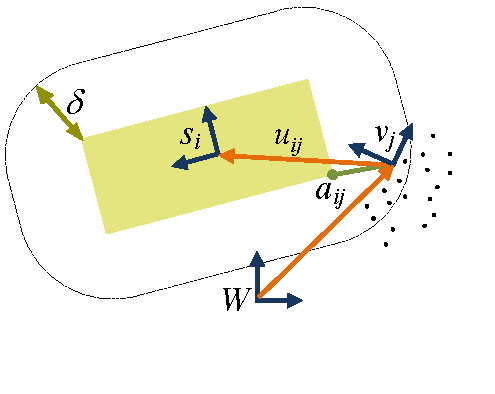
\includegraphics[width=5cm]{resources/model}}
\caption[Contact model]{Contact model. The figure shows the $i$-th link $\rl_i$ (solid block) and its pose $s_i$. The black dots are samples of the surface of an object. The distance $a_{ij}$ between a feature $v_j$ and the closest point on the link's surface is shown. The rounded rectangle illustrates the cut-off distance $\delta_i$. The poses $v_j$ and $s_i$ are expressed in the world frame $W$. The arrow $u_{ij}$ is the pose of $\rl_i$ relative to the frame for the surface feature $v_j$.}
\label{fig:representations.model}
\end{figure}

The parameters $\lambda$ and $\sigma_{p}$, $\sigma_{q}$, $\sigma_{r}$ were chosen empirically and kept fixed in all experiments reported in \sect\ref{sec:method}. The time complexity for learning each contact model from an example grasp is $\Omega(T K_O)$ where $T$ is the number of triangles in the tri-mesh describing the hand links, and $K_O$ is the number of points in the object model.


%\begin{figure}[t]
%\centering{
%\subfloat[]{\includegraphics[height=3.4cm]{resources/example1}}\quad
%\subfloat[]{\includegraphics[height=3.4cm]{resources/example2}}\quad
%\subfloat[]{\includegraphics[height=3.4cm]{resources/example5}}
%}
%\caption[Hand-object contact]{Example top grasp of a mug represented by a point cloud (panel a). The dotted regions are rays between features and the closest hand link surfaces (panel b). The black curves with frames at the fingertips represent the range of hand configurations in \eq\eqref{eq:hc} (panel c).}
%\label{fig:representations.modeldist.cont}
%\end{figure}

\subsection{Hand Configuration Model}

The hand configuration model, denoted by $\hc$, encodes a set of configurations of the hand joints $h_c \in \mathbb R^D$ (i.e., joint angles), that are particular to a grasp example. The purpose of this model is to allow us to restrict the grasp search space (during grasp transfer) to hand configurations that resemble those observed while training the grasp.

In order to boost the generalisation capability of the grasping algorithm the hand configuration model encodes the hand configuration that was observed when grasping the training object, but also a set of configurations recorded during the approach towards the object. Let us denote by $h^t_c$ the joint angles at some small distance \emph{before} the hand reached the training object, and by $h^g_c$ the hand joint angles at the time when the hand made contact with the training object. We consider a set of configurations interpolated between $h^t_c$ and $h^g_c$, and extrapolated beyond $h^g_c$, as
\begin{equation}
h_c(\gamma) = (1 - \gamma)h^g_c + \gamma h^t_c
\label{eq:learning.configmodel.config}
\end{equation}
\noindent where $\gamma \in \mathbb R$. For all $\gamma < 0$, configurations $h_c(\gamma)$ are beyond $h^g_c$ (see \fig\ref{fig:representations.modeldist.cont}). The hand configuration model $\hc$ is constructed by applying kernel density estimation to \begin{equation}\label{eq:H_c}\mathcal H_c = \lbrace h_c(\gamma): \gamma \in [-\beta, \beta], \beta \in \mathbb R^{+}\rbrace,\end{equation} as 
\begin{equation}
\hc(h_c) \equiv \sum_{\gamma \in [-\beta, \beta]} w({h_c(\gamma)}) \mathcal{N}_D(h_c|h_c(\gamma), \sigma_{h_c}) 
\label{eq:hc}
\end{equation}
where  $w({h_c(\gamma)}) = \exp(-\alpha \|h_c(\gamma) - h^g_c \|^2)$ and $\alpha \in \mathbb R^{+}$. $\alpha$ and $\beta$ were hand tuned and kept fixed in all the experiments. The hand configuration model computation has time complexity $\Omega(d_h K_C)$ where $d_h$ is the number of dimensions of the configuration vector, and $K_C$ is the size of the set of values of $\gamma$ used in \eq\eqref{eq:hc}.

\subsection{Reach to Grasp Trajectory}

We encode a reach to grasp trajectory as the combined trajectory of the wrist pose and the hand configuration. Each wrist pose is defined in the frame of reference of the final wrist pose in the trajectory. This final wrist pose is associated with the final hand configuration model and the contact models. We refer to the final hand configuration model, wrist pose and contact models as the model of the final grasp state.  A set of reach to grasp trajectories, including the final grasp states can be defined. We create this set so that the final grasp states are all very close to one another, thus forming an attractor, with the trajectories leading to those similar final grasp states defining an attractor basin.


\section{LEARNING}
% SAY HOW WE USE THE SIMULATOR HERE
% DESCRIBE BRIEFLY THE HAND

There are several ways to implement underactuation in a humanoid hand. We are particularly intereseted in the adaptive synergy transmission due to its simplicity and robust design, yet complex interaction with the environment. The Pisa/IIT SoftHand~\cite{Catalano2014Adaptive} exhibits one of such transmissions.

The hand has 19 degrees of freedom distributed in four fingers and an opposable thumb, and only 1 degree of actuation. The synergy motion derives from human postural databases. The overall behavior parameters are the matrices that correspond to the transmission ratio,~$R$, to the joint stiffness,~$K_q$. The actuation is done through a single tendon routed throuhout all joints, making the fingers to flect and abduct.

% THE LACK OF SENSORS AND FUTURE LARGE DATASETS REQUIRED JUSTIFY THE USE OF SIMULATED DATA

Moving such a hand to grasp an object results in a hard-to-predeict contact and hand shapes due to the adaptivity. To the purpose of this work, we are intereseted in generating examples of this kind. However, recording the trajectory of all bodies into play in a real scenario is not a banal thing when dealing with cluttered and small spaces where human-sized grasps take place, specially if hundreds are required. For this reason, we have opted to generate the examples using a rigid-body dynamic simulator, where these problems are overcome, however, others arise. The main two elements are the contact stability and the hand behavior, which in this case, the latter depends heavily on the former. We are using the standard distribution of Gazebo and Open Dynamic Engine, both widely spread with recognized performance.
%% but not perfect. There is an on-going work on improving the mesh-to-mesh collision there.
Regarding the second element, the adaptive synergy equations have been implemented as a plugin which accompanies the proper kinematic description of the Pisa/IIT SoftHand\footnote{The Pisa/IIT SoftHand ROS/Gazebo packages are available at \url{https://github.com/CentroEPiaggio/pisa-iit-soft-hand}}.
%
%\begin{figure}
%  \centering
%  \begin{tabular}{ccc}
%
%  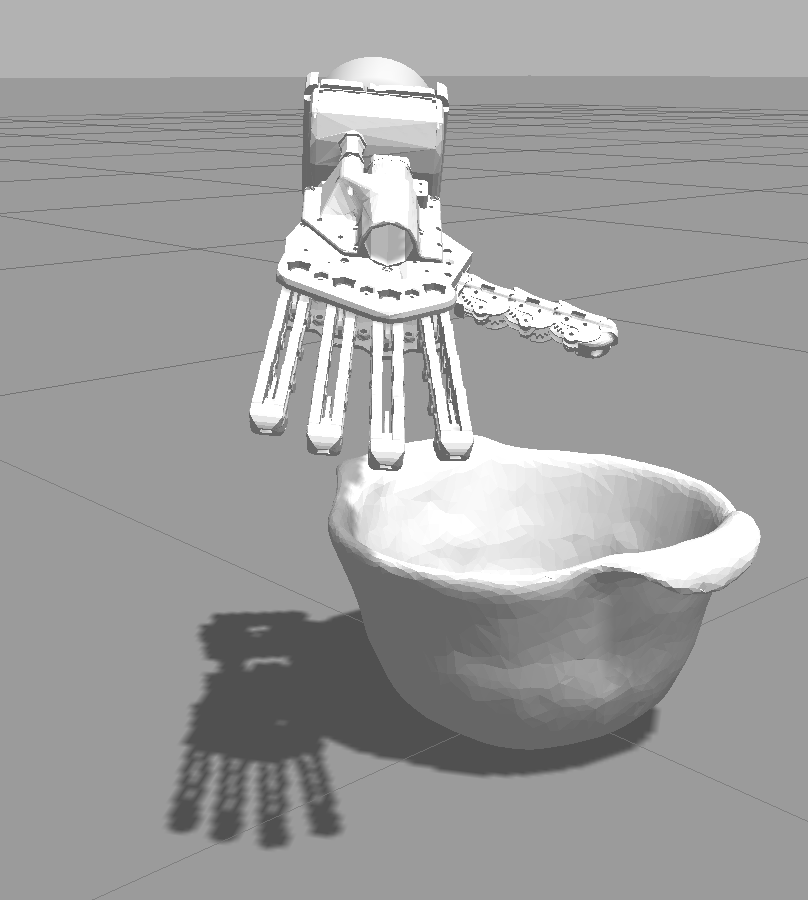
\includegraphics[width=0.3\linewidth]{containerB_pinch_1.png} &
%
%  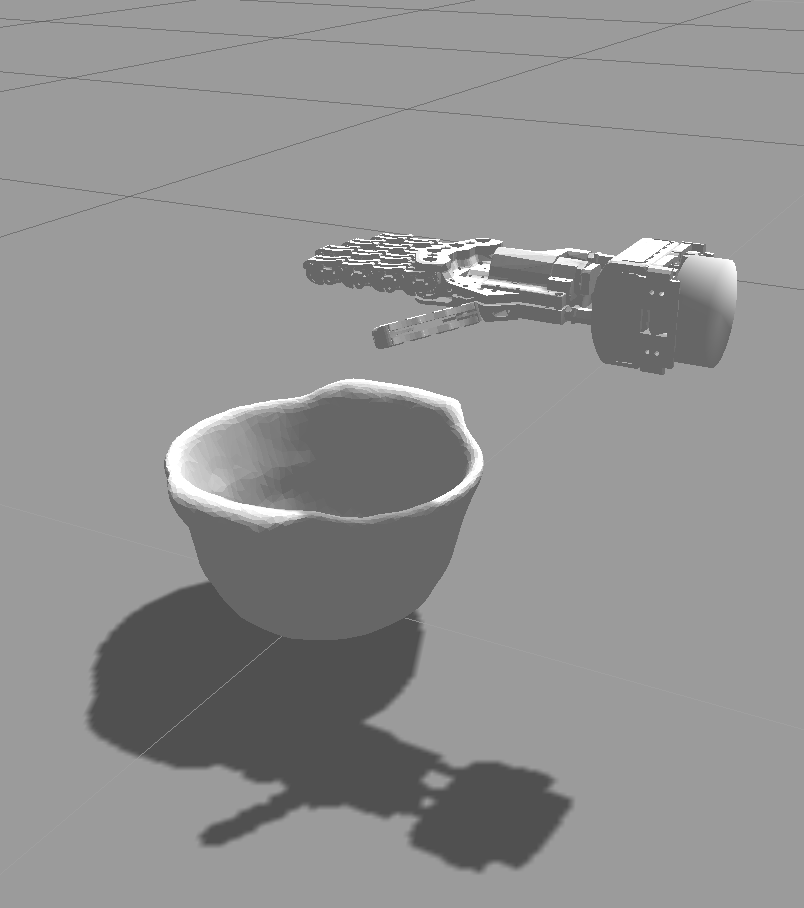
\includegraphics[width=0.3\linewidth]{containerB_rim_1.png} &
%
%  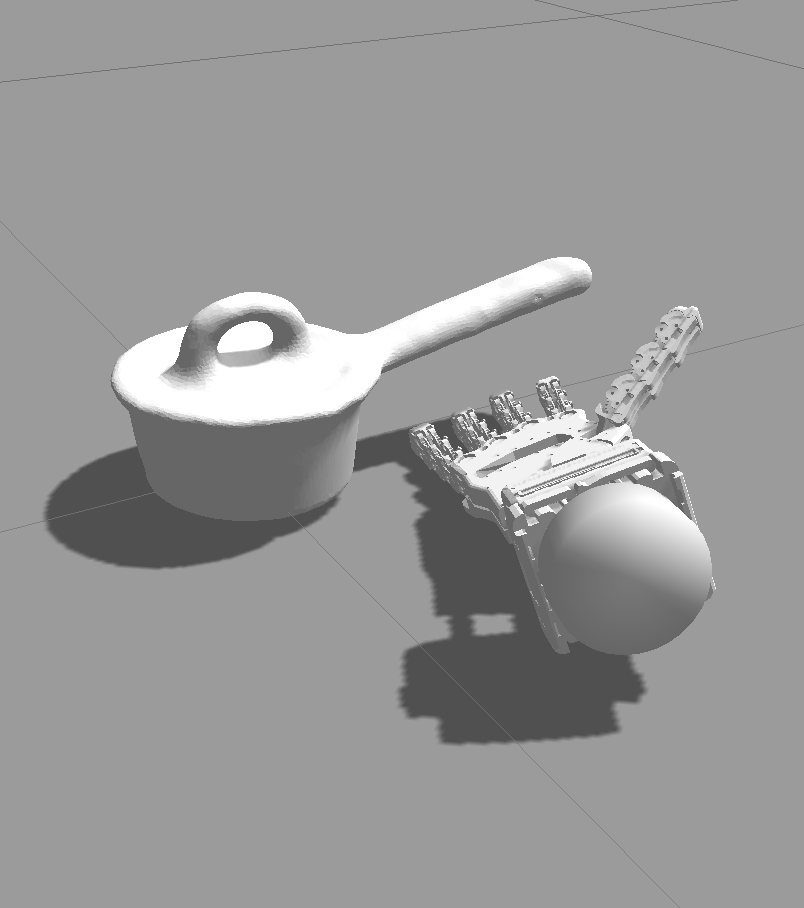
\includegraphics[width=0.3\linewidth]{pot_1.png} \\
%
%  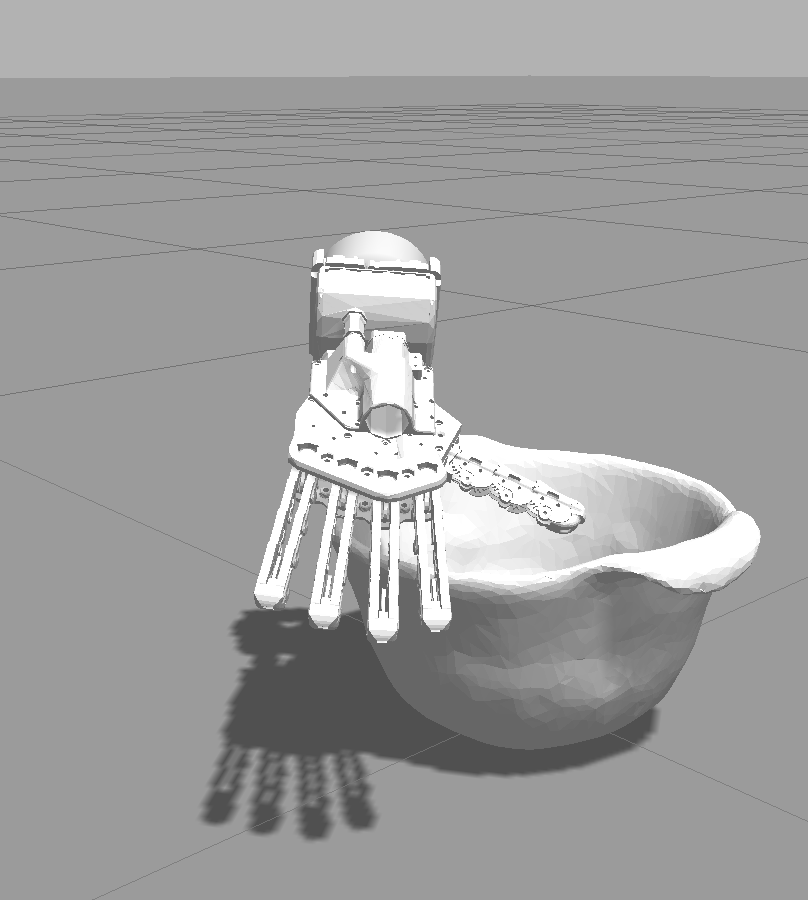
\includegraphics[width=0.3\linewidth]{containerB_pinch_2.png} &
%
%  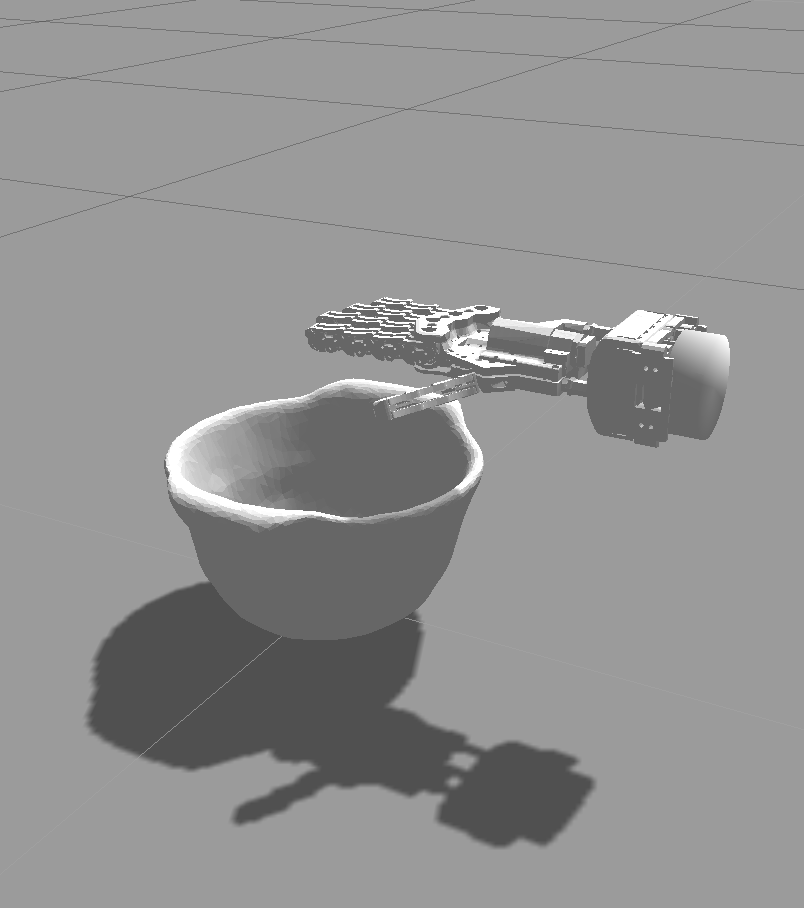
\includegraphics[width=0.3\linewidth]{containerB_rim_2.png} &
%
%  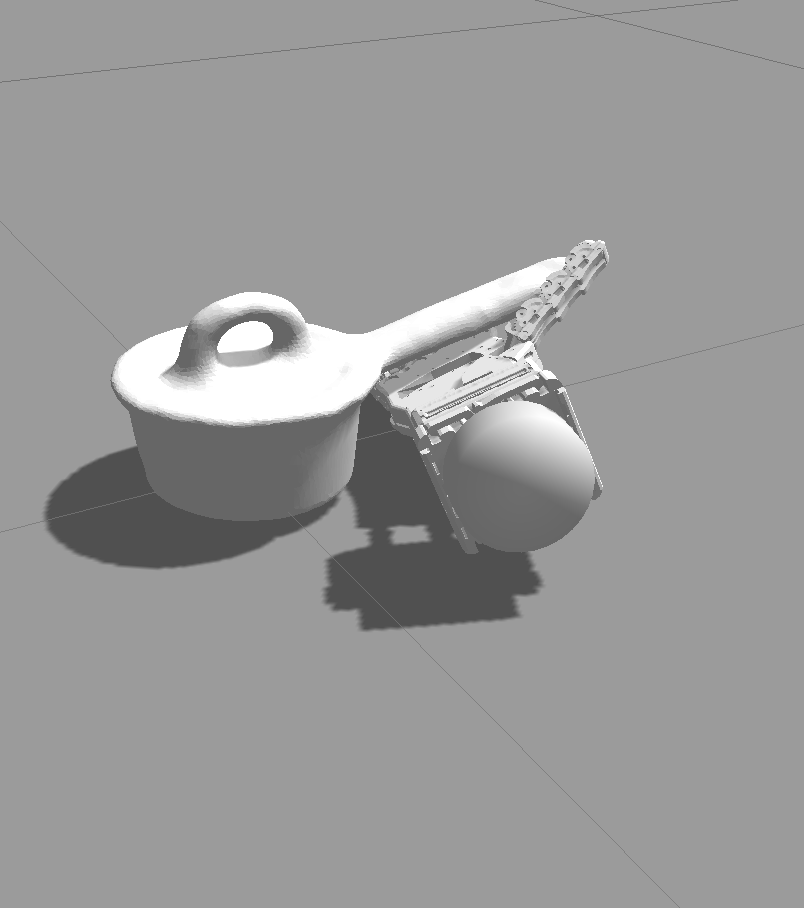
\includegraphics[width=0.3\linewidth]{pot_2.png} \\
%
%  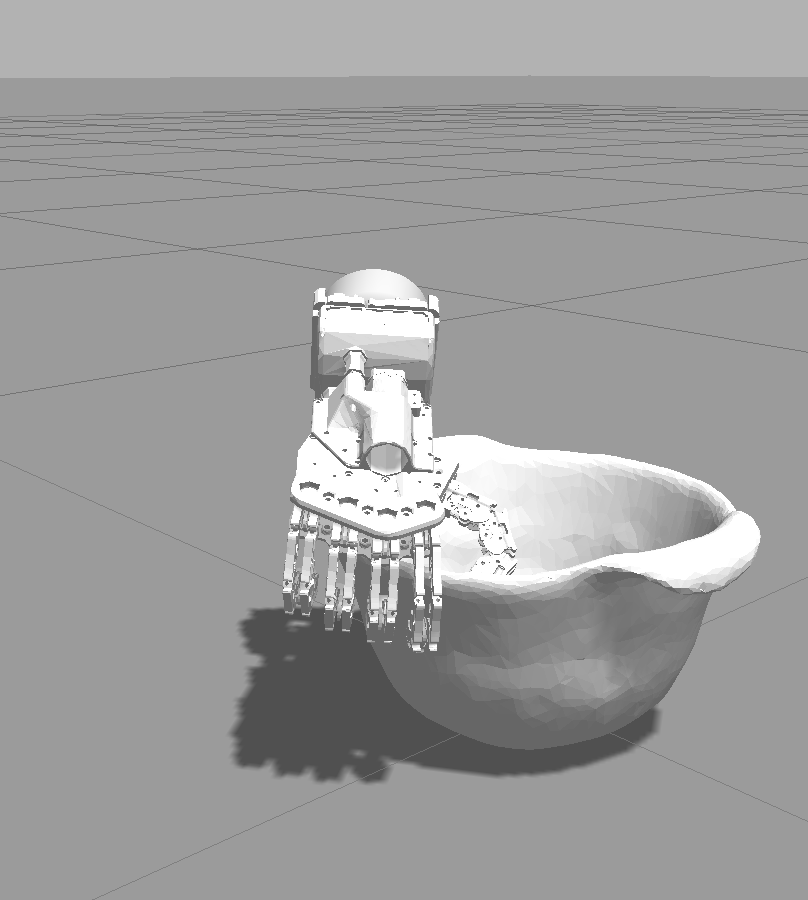
\includegraphics[width=0.3\linewidth]{containerB_pinch_4.png} &
%
%  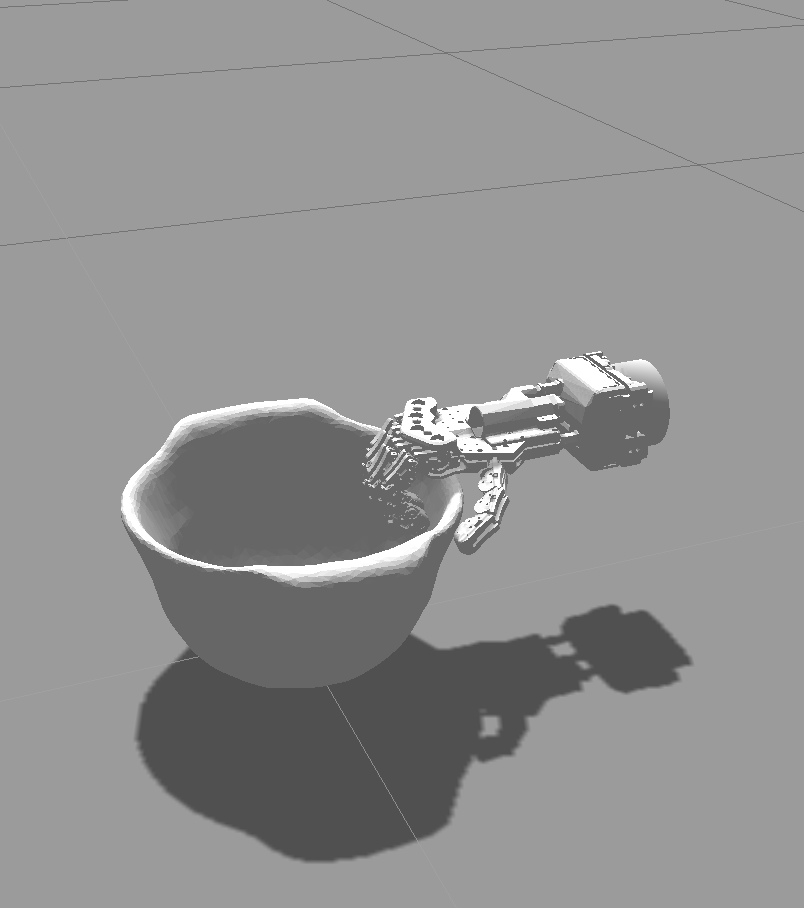
\includegraphics[width=0.3\linewidth]{containerB_rim_4.png} &
%
%  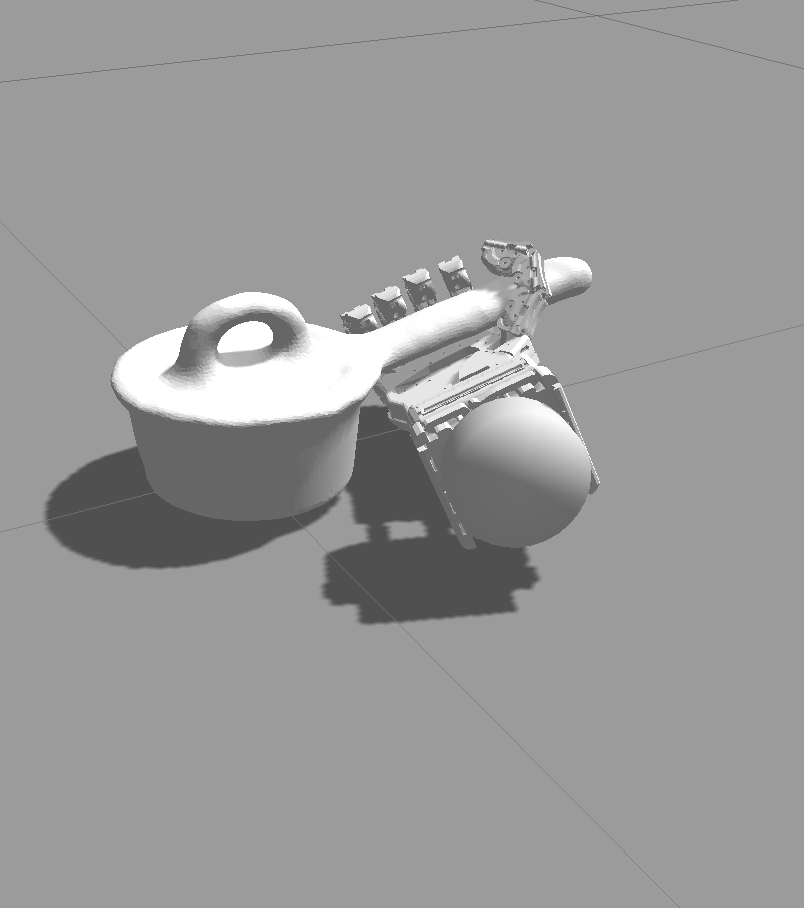
\includegraphics[width=0.3\linewidth]{pot_3.png} \\
%
%  \end{tabular}
%
%  \caption{Snapshots of the simulation of a pinch and rim grasp types for the colander (first and second columns), and handle grasp for the pot (last column).}
%  \label{fig:simulations}
%\end{figure}
%
%% HOW WE GENERATED THE DATA
%
At the current state, there are no generally accepted measures concerning whether an object being grasped by an underactuated adaptive hand  is good or not, hence the lack of robust grasp planners for them is not a surprise. Thus, generating a large dataset at this point is useless, and there are plans in the future to cover this area. As a result, we generated the examples by guiding manually the hand to a ``nice'' grasp as shown in Fig.~\ref{fig:simulations}. In this simpler scenario, we assume without lost of generality that the grasps are labeled by type. In our example dataset, we have three grasp types namely pinch, rim and by-the-handle. The main difference between pinch and rim is the fingers configuration w.r.t. the top border of objects. In the pinch grasp, the thumb goes inside whereas in the rim grasp, the fingers go inside. In the latter, the container can be filled with liquid while holding, for instance.
%
For each grasp example, the corresponding dataset comprises the set of trajectories as described above.

%For each grasp example, the corresponding dataset comprises the set of body trajectories, expicitly their position, $p_i(t) \in \mathbb{R}^3$, and orientation, $q_i(t) \in SO(3)$, over time for $i=1 , \ldots , m$ bodies (including hand links), and an associated set of hand configurations, $h_c(t) \in R^{n}$, with $n$ the hand degrees of freedom.
%%associated set of hand configurations, %$h_c(t) \in R^{n}$, with $n$ the hand degrees of freedom.

% FOR FUTURE WORK?

% Another challenge is to learn how any adaptive synergy transmission behave for any given kinematic design. 

%% BECAUSE I'M WORKING IN GENERATING DATA FOR ANOTHER COMPLIANT HAND BESIDES THE PISA SOFTHAND

\section{INFERENCE}
\label{sec:infer}
% NEED TO ADAPT FOR SOFT HAND (TRAJECTORY + CONTACT MODEL)

After acquiring the models from a set of training grasps, we present the robot with a test (query) object. The goal is to find a generalisation of the training grasp that is likely according to all of the model types simultaneously. First of all, we obtain a point cloud for the test object, and thus an object model. We then combine every contact model with that object model, so as to obtain a set of {\em query densities}, one for each link with a contact model defined for the example grasp. The $i$-th query density $\qd_i$ is a density modelling where the $i$-th link can be placed, in the equilibrium state, with respect to the surface of a new object. 

From the query densities, a candidate equilibrium grasp state is generated as follows. We randomly pick a link $i$. We randomly sample, from the corresponding query density $\qd_i$, a pose for link $i$. We sample, from the configuration model $\hc$, a final hand configuration that is compatible with the pose selected for link $i$, and then we compute from forward kinematics the poses of all the remaining hand links. This defines a candidate equilibrium grasp state. This is then augmented with a reach to grasp trajectory that will lead to it. The reach to grasp trajectory is selected that finishes closest to the candidate equilibrium grasp state. Finally we refine the equilibrium grasp and reach to grasp by performing a simulated annealing search in the space of equilibrium state wrist poses and hand configurations, so as to maximise the grasp likelihood. Grasp likelihood is the product of the hand configuration density, the reach to grasp density, and the query densities for all the hand links. We repeat the entire process a number of times. The optimisation procedure generates many possible grasps, each with its likelihood. The following subsections explain how to estimate query densities, and how grasp optimisation is carried out.

\subsection{Query Density Computation}

A query density \eqref{eq:qd} is expressed, for a hand link and an object model, as a density for the pose of that hand link relative to the object. Intuitively the query density encourages a finger link to make contact with the object at locations that have similar local surface curvature to that in the training example. Specifically, we use $K_{Q_i}$ kernels centred on the set of weighted finger link poses:
\begin{equation}
\qd_i(s) \simeq \sum^{K_{Q_i}}_{j=1} w_{ij} \mathcal{N}_3(p|{\hat{p}_{ij}}, \sigma_{p}) \Theta(q|{\hat{q}_{ij}}, \sigma_{q})%, \quad i = 1, ..., N_L
\label{eq:qd.approx}
\end{equation}
with $j$-th kernel centre $({\hat{p}_{ij}}, {\hat{q}_{ij}}) = \hat{s}_{ij}$, and where all weights were normalised $\sum_j w_{ij} = 1$. When a test object is presented, a set of query densities $\mathcal{Q}^g$ is calculated for the equilibrium state for each training grasp $g$. The set $\mathcal{Q}^g =\{\qd_i^g\}$ has $N^g_Q=N^g_M$ members, one for each contact model $M_i^g$ in $\mathcal{M}^g$.

\section{Inferring Grasps for Novel Objects}
\label{sec:infernovel}
\input{./inputTex/novelobjects.tex}

\section{RESULTS}
\label{sec:results}
% DESCRIBE EXPERIMENTS
The experiments were conducted as follows. Training consisted of nine example grasps, executed in simulation, with a human in control. These nine grasps were grouped into three grasp types (rim, pinch, and handle). The rim and pinch grasp types were trained on the colander object, and the handle grasp type was demonstrated on the saucepan. During testing an object was placed on the table. Every grasp type was compared automatically, and one selected for execution according to the methods described above. The models of the test objects consisted of a point cloud taken from just one view. Thus reconstructions were partial, typically less that 25\% of the object's surface area. No test objects had been seen previously by the robot, and it can be seen from Fig.~\ref{fig:test}. Fifteen test objects were presented, and 12 of the 15 test grasps succeeded, giving a generalisation success rate of 80\%. While the difference is not statistically significant, this is slightly higher than the 77.7\% success rate we recorded on a larger test set for a fully actuated hand also working from a single view of an object \cite{kopicki-detry-wyatt-etal-ijrr-2015}.

It is worth noting the similiarity between the location of the actual and targetted final grasp states. In a majority of cases the grasp involved interactions with the object, moving it to the stable grasp pose. This is a natural property of the hand, but it might have been supposed that the learning method would not be robust to such interactions in terms of the accuracy of the grasp. 

\begin{figure}
\begin{center}
 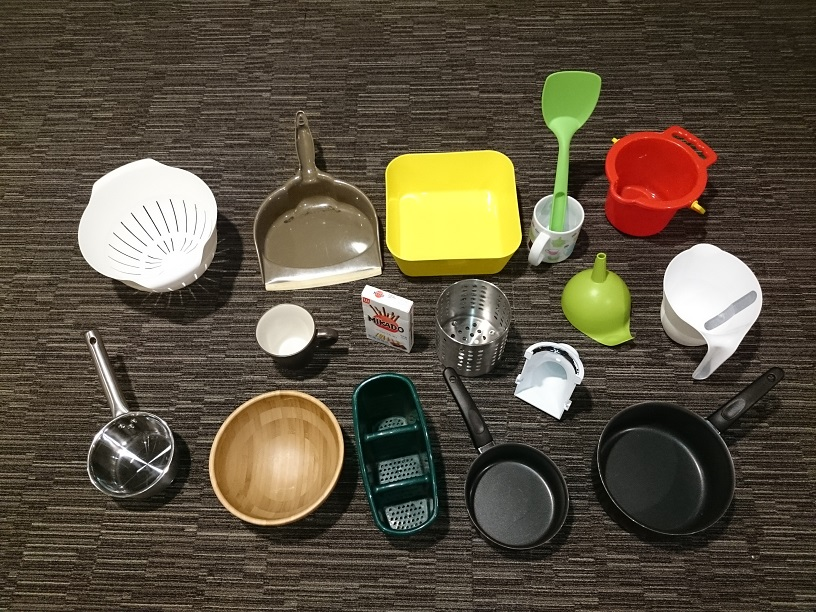
\includegraphics[width=0.9\columnwidth]{images/object_set_small}
 \caption{The two training objects are on the far left. The testing objects on the right. 12 from 15 test grasps on novel objects were successful.}
 \label{fig:test}
 \end{center}
\end{figure}

\begin{figure*}
\begin{center}
\newcommand{\tw}{0.15\linewidth}
 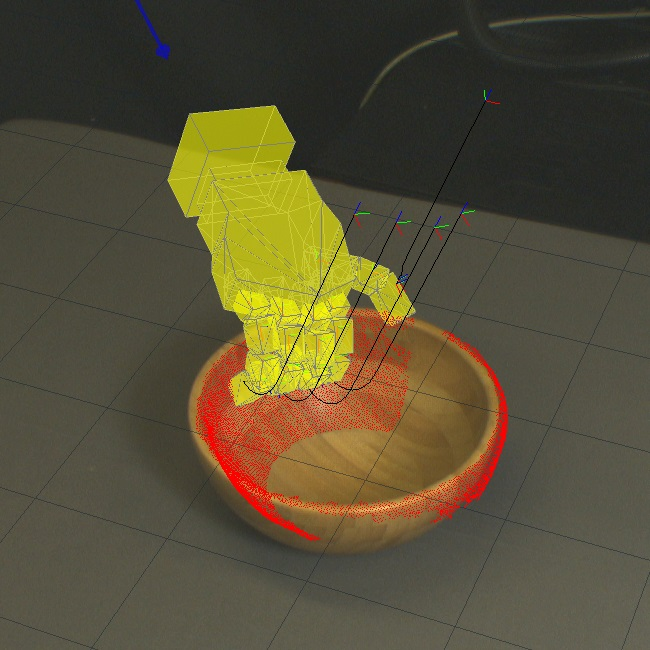
\includegraphics[width=\tw]{images/experiments/query/bowllarge-1-s}
 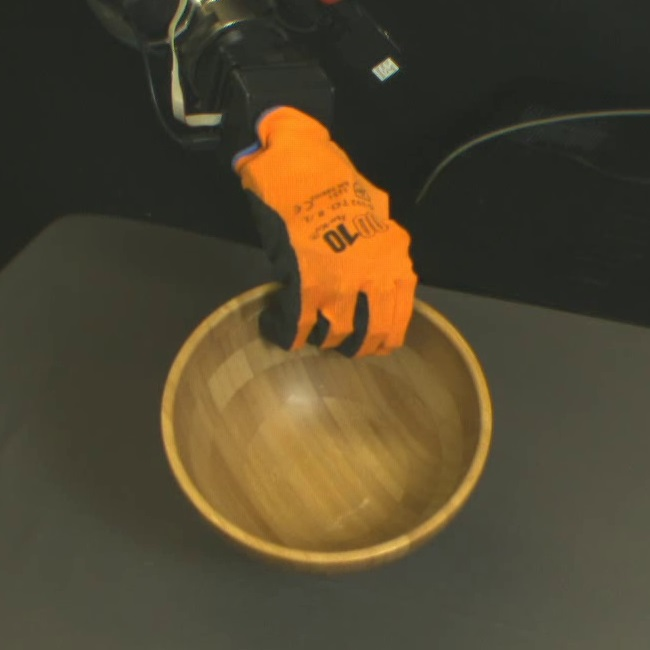
\includegraphics[width=\tw]{images/experiments/exec/bowllarge-s}
 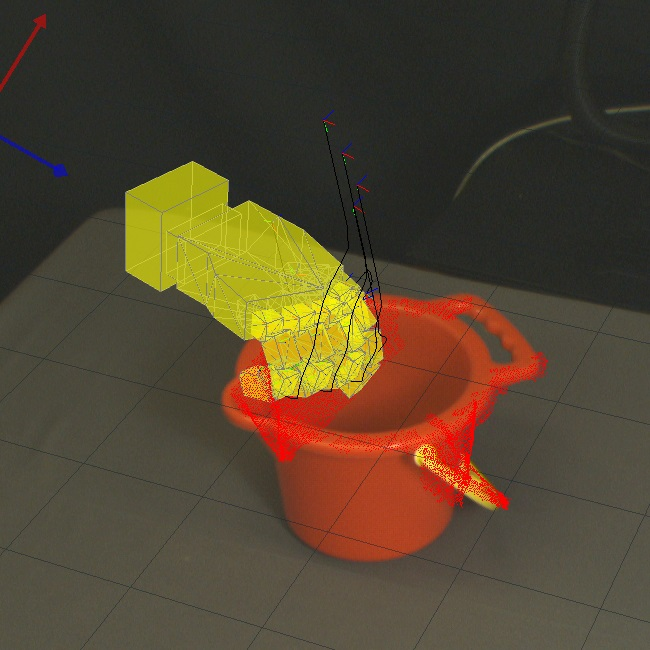
\includegraphics[width=\tw]{images/experiments/query/bucket-1-s}
 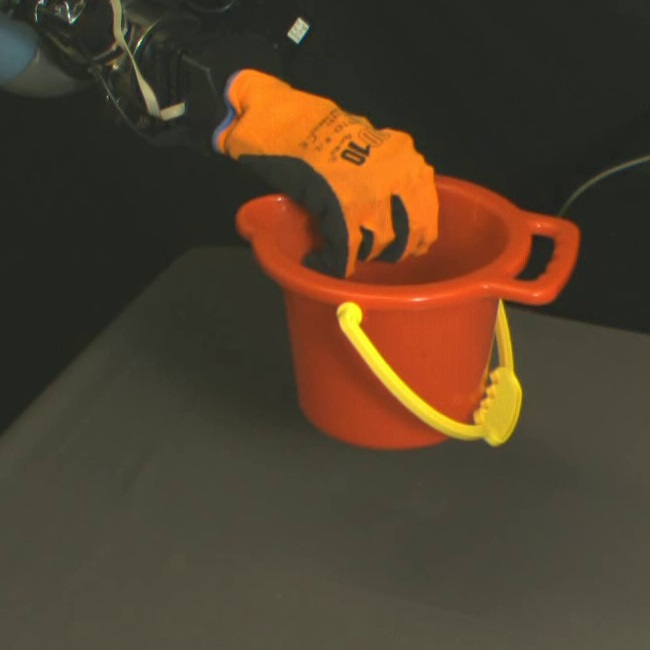
\includegraphics[width=\tw]{images/experiments/exec/bucket-s}
  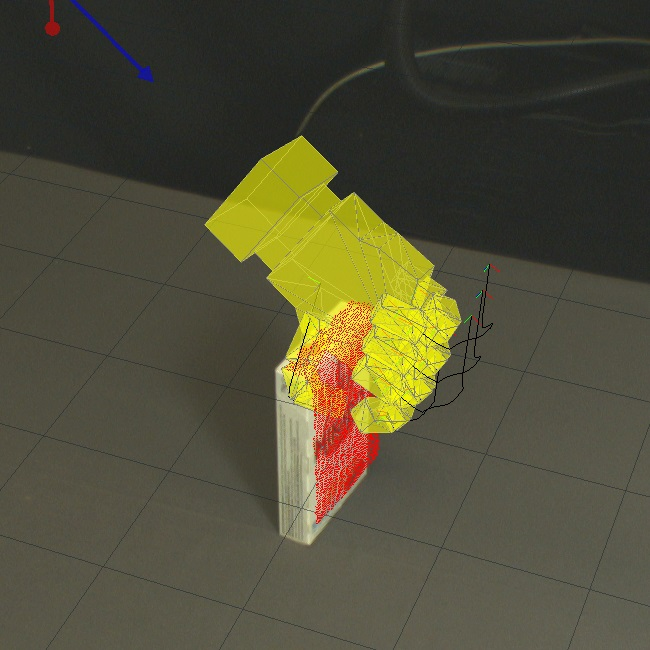
\includegraphics[width=\tw]{images/experiments/query/chocsticks-1-s}
 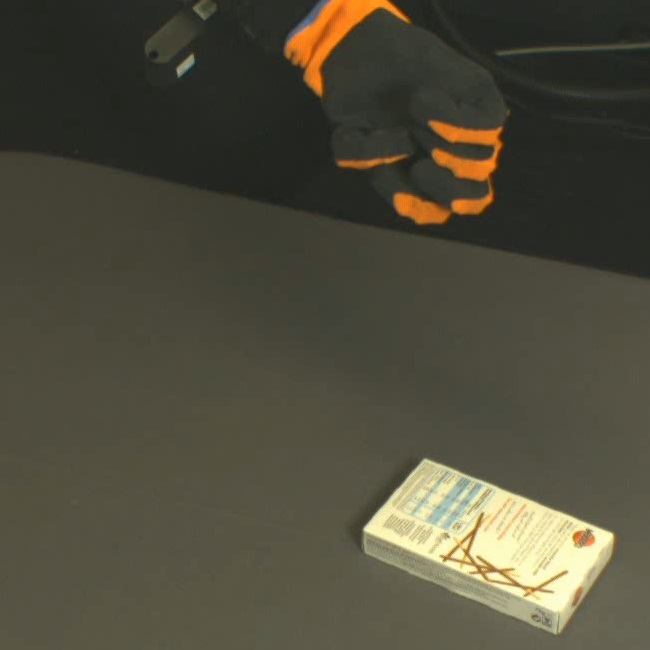
\includegraphics[width=\tw]{images/experiments/exec/chocsticks-s}\\
  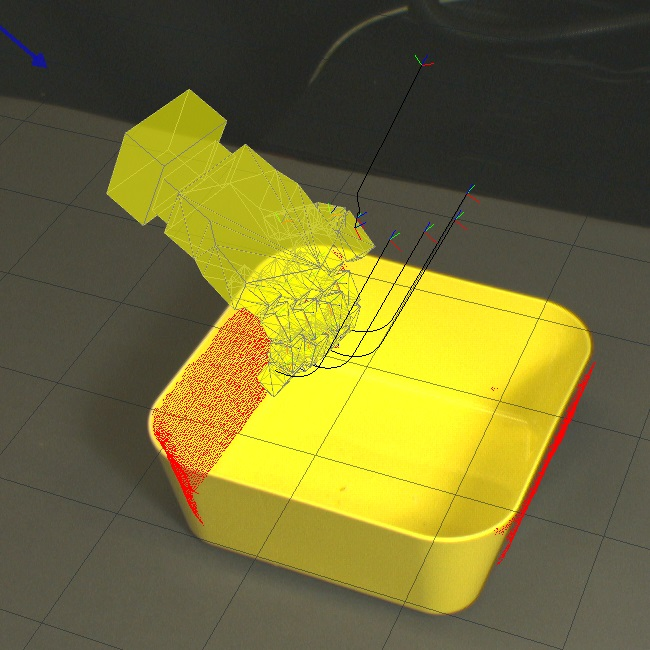
\includegraphics[width=\tw]{images/experiments/query/container1-1-s}
 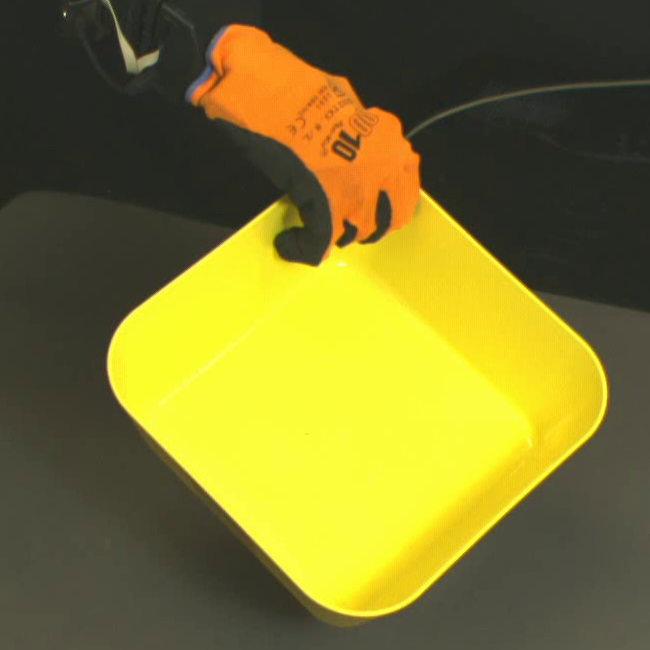
\includegraphics[width=\tw]{images/experiments/exec/container1-s}
  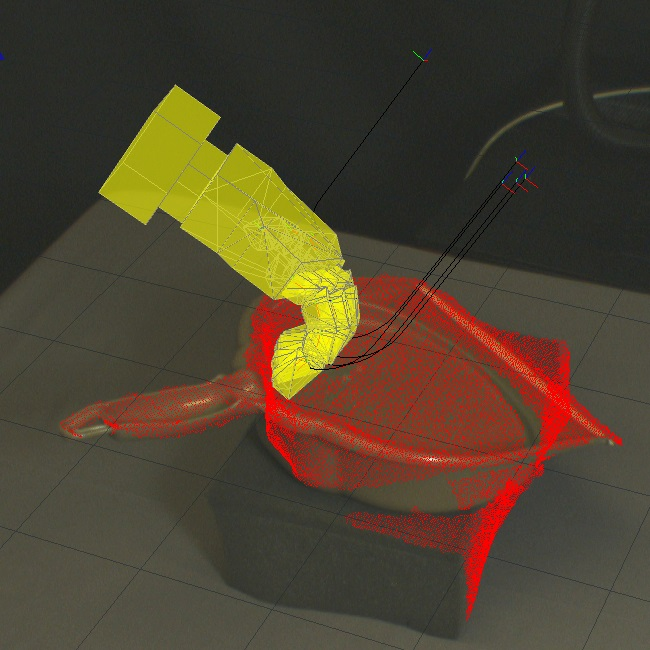
\includegraphics[width=\tw]{images/experiments/query/dustpan-1-s}
 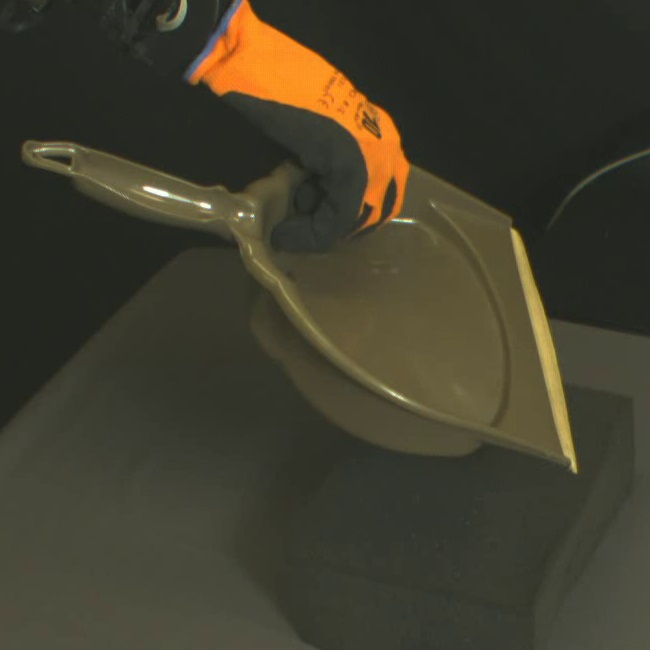
\includegraphics[width=\tw]{images/experiments/exec/dustpan-s}
  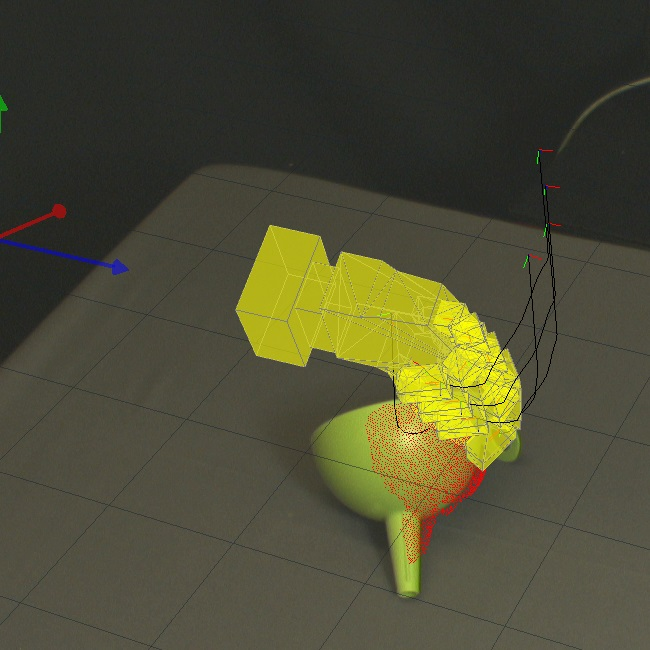
\includegraphics[width=\tw]{images/experiments/query/funnellarge-1-s}
 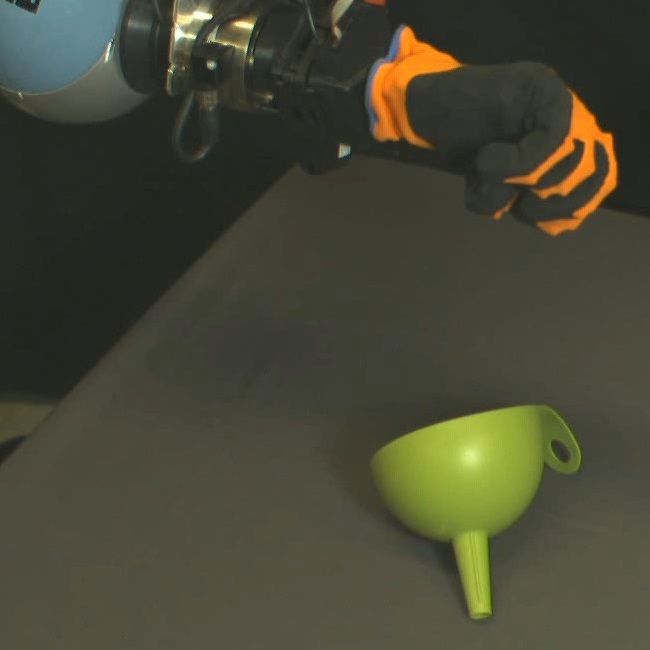
\includegraphics[width=\tw]{images/experiments/exec/funnellarge-s}\\
  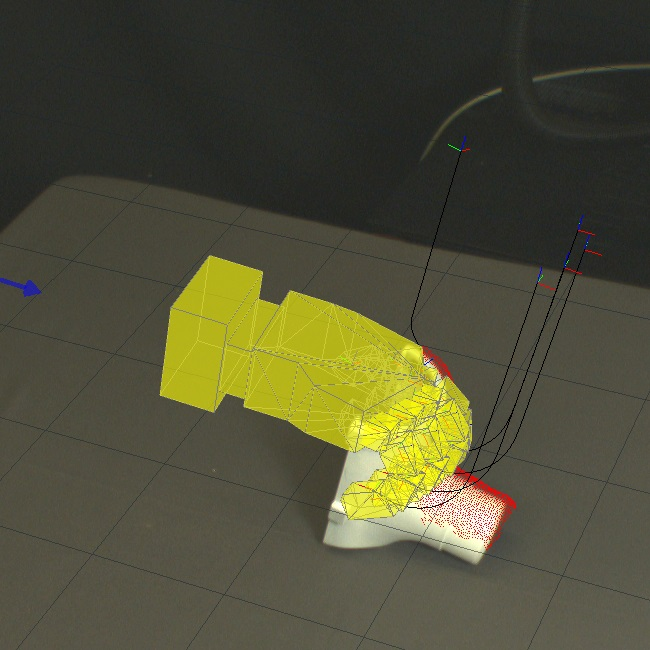
\includegraphics[width=\tw]{images/experiments/query/guttering-1-s}
 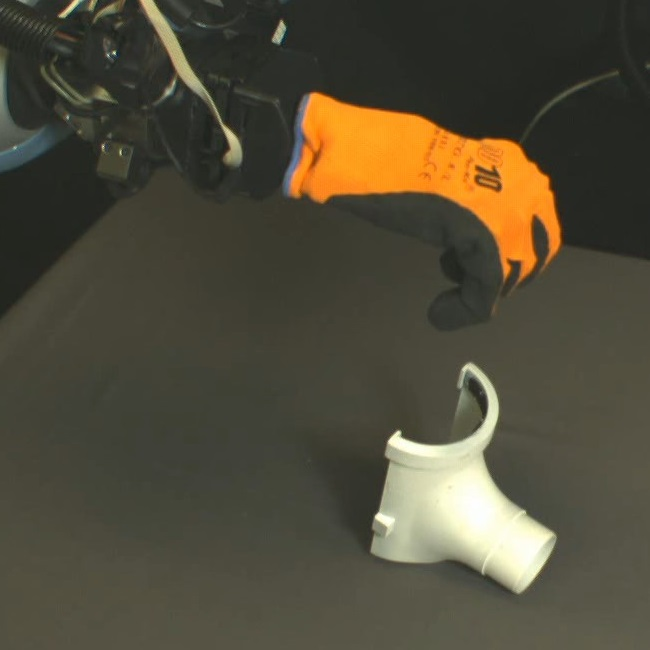
\includegraphics[width=\tw]{images/experiments/exec/guttering-s}
  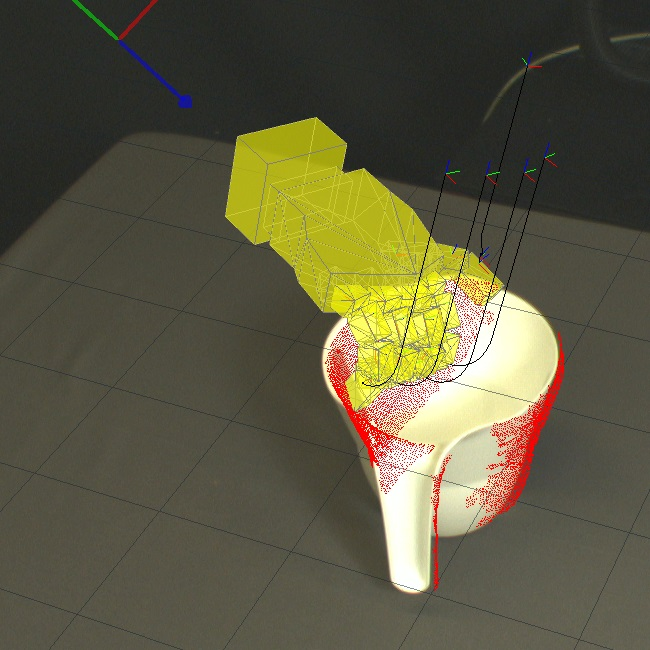
\includegraphics[width=\tw]{images/experiments/query/jug-1-s}
 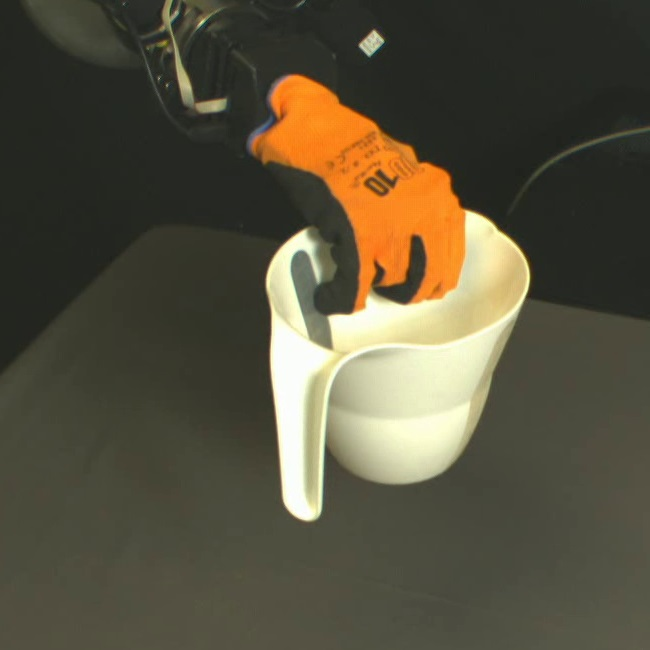
\includegraphics[width=\tw]{images/experiments/exec/jug-s}
  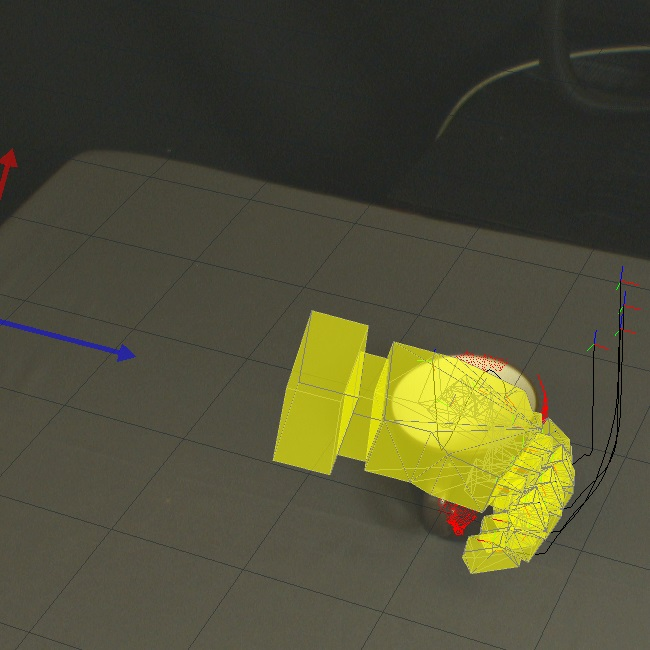
\includegraphics[width=\tw]{images/experiments/query/mug1-1-s}
 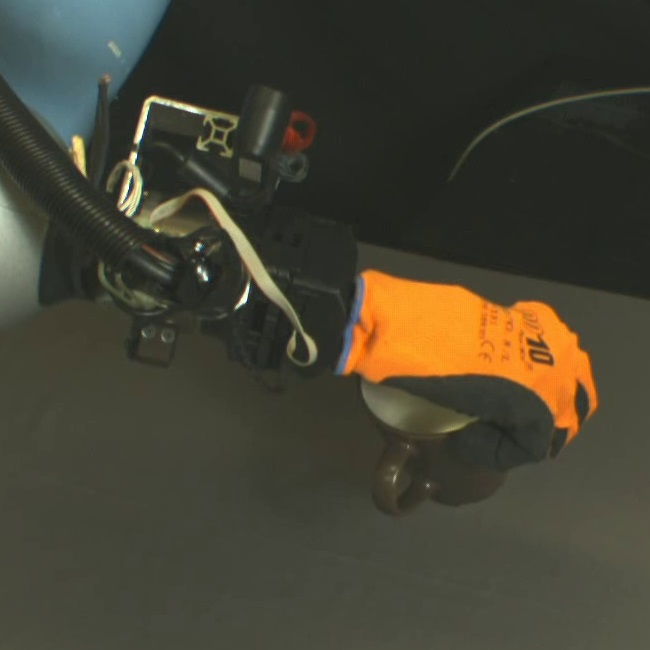
\includegraphics[width=\tw]{images/experiments/exec/mug1-s}\\
  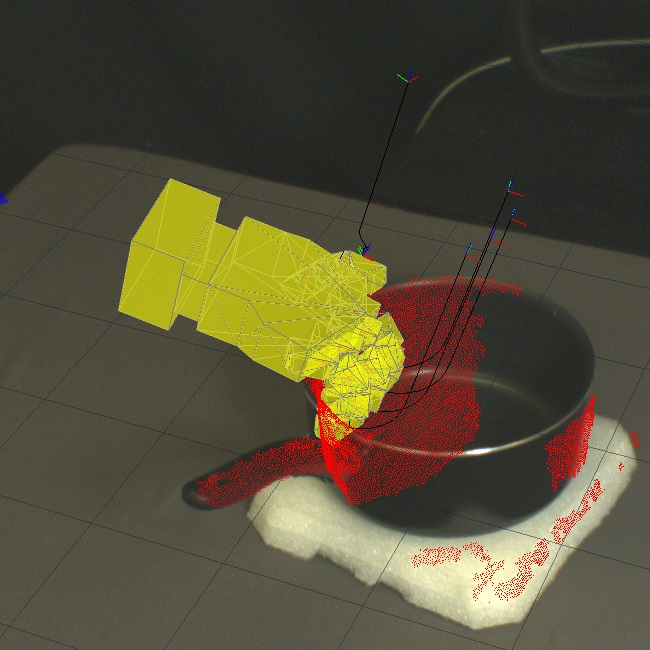
\includegraphics[width=\tw]{images/experiments/query/saucepanlarge-1-s}
 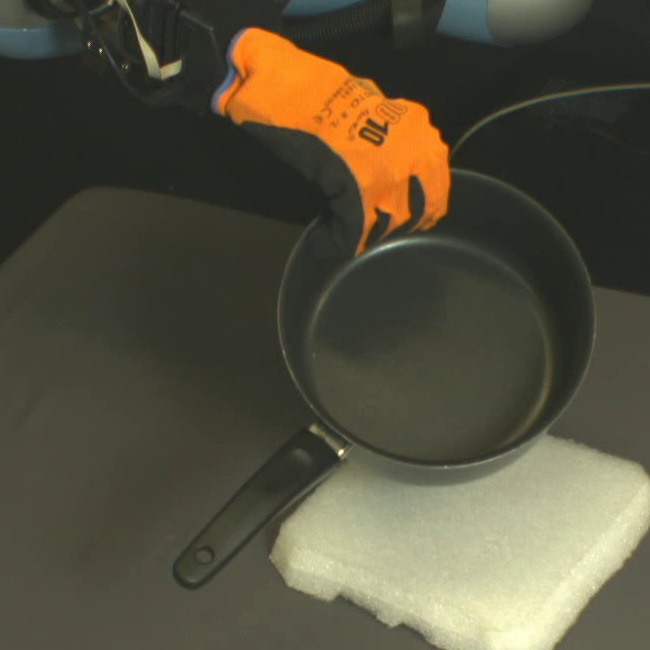
\includegraphics[width=\tw]{images/experiments/exec/saucepanlarge-s}
  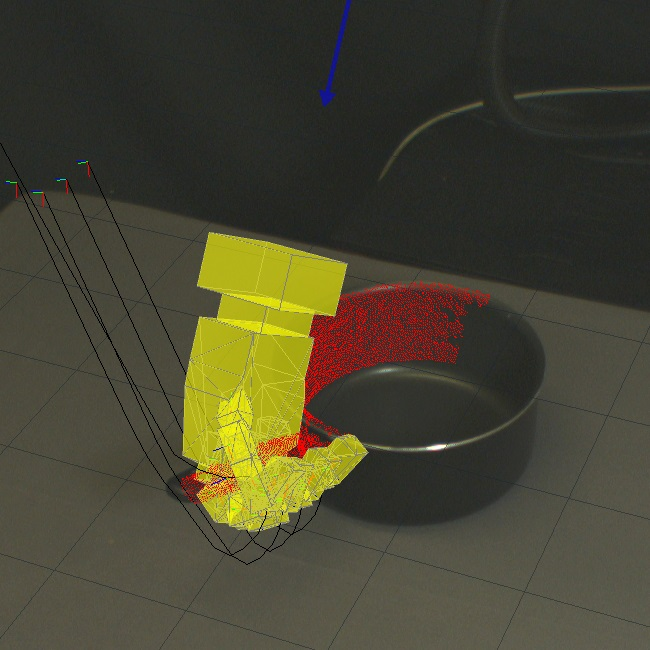
\includegraphics[width=\tw]{images/experiments/query/saucepanlarge-handle-1-s}
 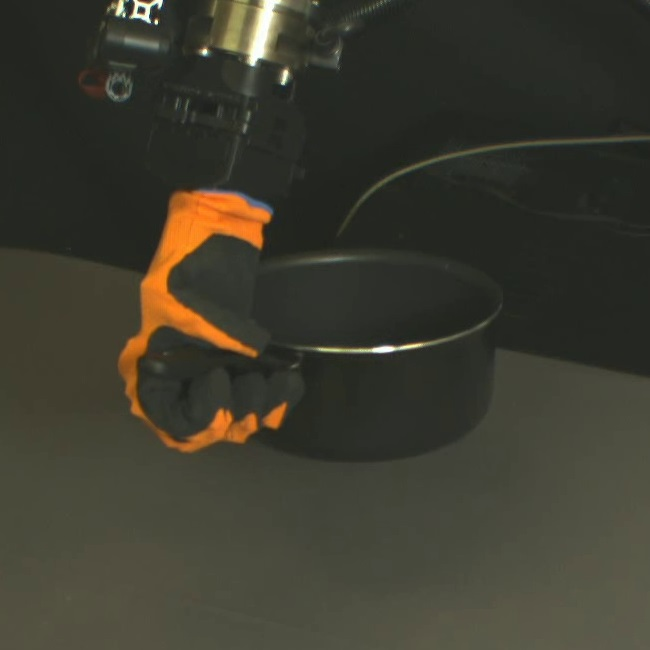
\includegraphics[width=\tw]{images/experiments/exec/saucepanlarge-handle-s}
  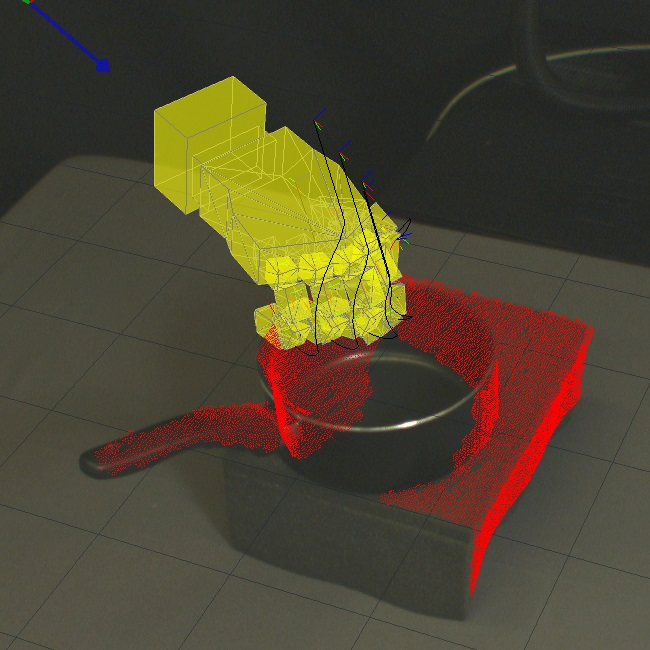
\includegraphics[width=\tw]{images/experiments/query/saucepansmall-1-s}
 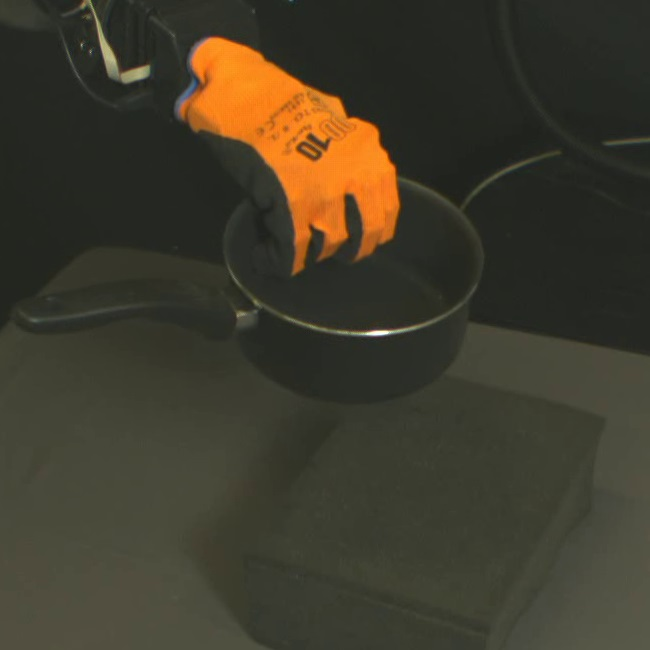
\includegraphics[width=\tw]{images/experiments/exec/saucepansmall-s}\\
  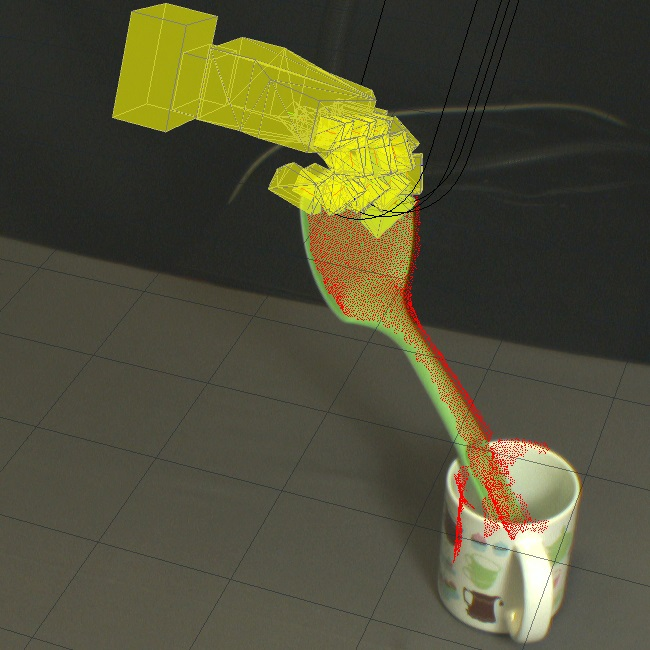
\includegraphics[width=\tw]{images/experiments/query/spatula-1-s}
 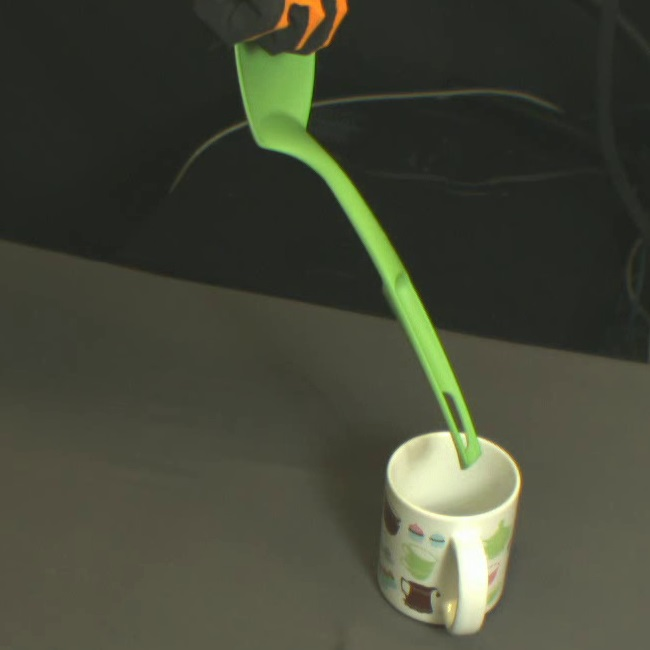
\includegraphics[width=\tw]{images/experiments/exec/spatula-s}
  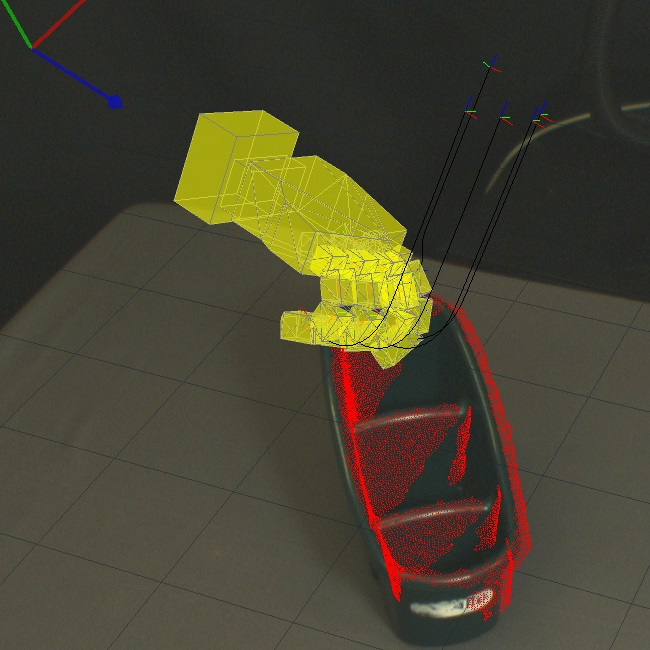
\includegraphics[width=\tw]{images/experiments/query/stand1-1-s}
 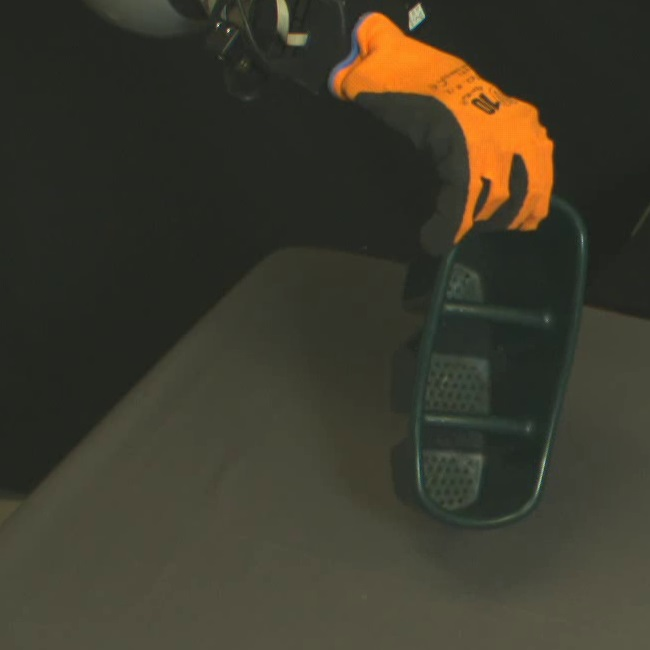
\includegraphics[width=\tw]{images/experiments/exec/stand1-s}
  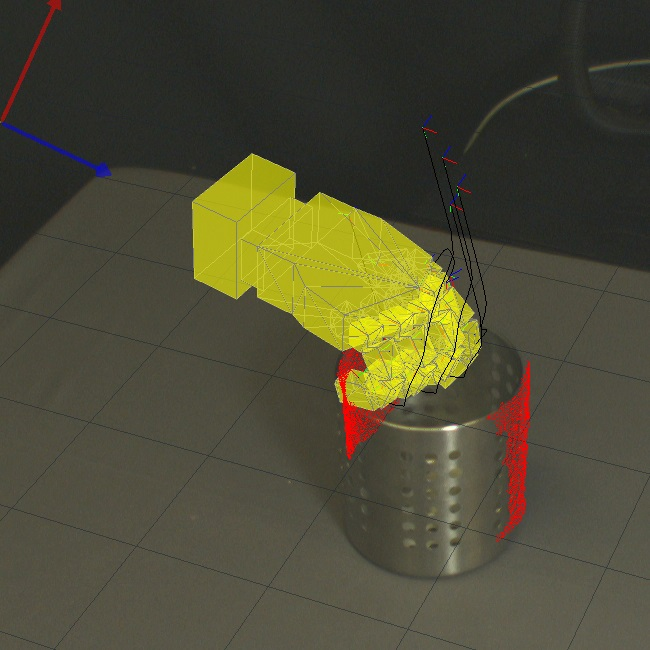
\includegraphics[width=\tw]{images/experiments/query/stand2-1-s}
 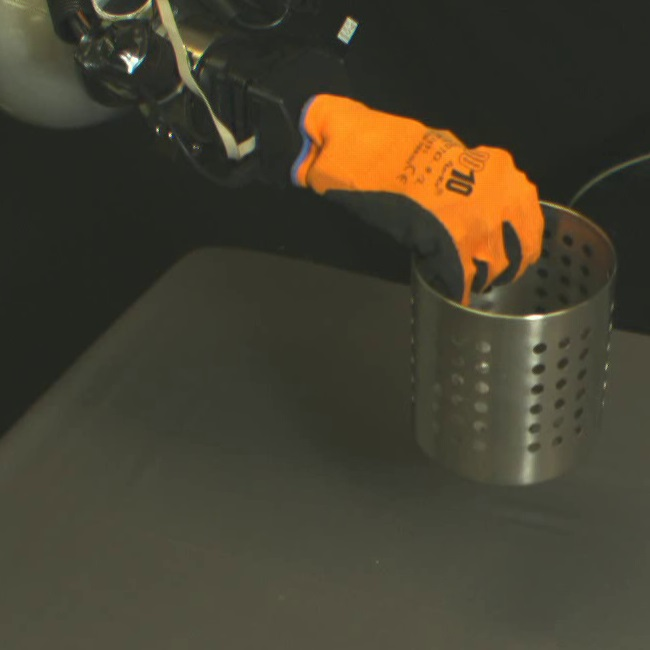
\includegraphics[width=\tw]{images/experiments/exec/stand2-s}
 \caption{The fifteen test grasps. Each one has a pair of images. The predicted equilibrium grasp state is shown on the left of each pair, and the actual grasp on the right. Counting from top left it can be seen that grasps 3,6, and 7 failed. All other grasps succeeded.}
 \label{fig:test}
 \end{center}
\end{figure*}



 

%%%%%%%%%%%%%%%%%%%%%%%%%%%%%%%%%%%%%%%%%%%%%%%%%%%%%%%%%%%%%%%%%%%%%%%%%%%%%%%%
\bibliographystyle{IEEEtran}
%\bibliography{bibliography/carlos,bibliography/ref1,bibliography/ref2}
%% THERE ARE REPEATED ENTRIES IN REF1 AND REF2
\bibliography{bibliography/carlos,bibliography/ref1}

\addtolength{\textheight}{-12cm}

%\section*{APPENDIX}
%
%
%\section*{ACKNOWLEDGMENT}


\end{document}
